\documentclass[11pt,a4paper]{article}

% Packages
\usepackage[margin=1in]{geometry}
\usepackage{graphicx}
\usepackage{amsmath}
\usepackage{amssymb}
\usepackage{natbib}
\usepackage{hyperref}
\usepackage{booktabs}
\usepackage{array}
\usepackage{xcolor}
\usepackage{float}
\usepackage{caption}
\usepackage{subcaption}

% Title and metadata
\title{\textbf{Multi-Task Machine Learning for Predicting ADMET Properties: A Comprehensive Approach Combining Gradient Boosting and Graph Neural Networks}}

\author{K-Dense web}

\date{December 5, 2025}

\begin{document}

\maketitle

\begin{abstract}
Accurate prediction of Absorption, Distribution, Metabolism, Excretion, and Toxicity (ADMET) properties is critical for accelerating drug discovery and reducing late-stage attrition rates. In this study, we developed and validated multi-task machine learning models for predicting nine key ADMET endpoints using the OpenADMET-ExpansionRx blind challenge dataset comprising 5,326 training molecules and 2,282 blind test compounds. We implemented a dual-track modeling strategy combining traditional gradient boosting (LightGBM) with molecular fingerprints and descriptors, alongside advanced multi-task neural networks with Z-score normalized targets. Our baseline LightGBM models achieved a mean Spearman correlation of 0.7682 across all nine endpoints, while the multi-task neural network approach improved performance to 0.7779 Spearman (mean MA-RAE: 0.5481). The multi-task learning framework demonstrated particular efficacy for sparse endpoints, with the sparsest property (MGMB, 95.8\% missing data) showing a 16.85\% improvement in Spearman correlation. Our analysis revealed hierarchical missingness patterns (3.7--95.8\%), strong inter-property correlations (MBPB-MGMB: r=0.904), and distribution shifts between training and test sets. The ensemble approach combining both modeling strategies yielded robust predictions for all test molecules. These results demonstrate that thoughtful application of target normalization, scaffold-based validation, and multi-task learning can achieve near state-of-the-art performance in ADMET prediction while maintaining computational efficiency.
\end{abstract}

\section{Introduction}

\subsection{Background and Significance}

The pharmaceutical industry faces substantial challenges in drug development, with approximately 90\% of drug candidates failing during clinical trials, often due to poor pharmacokinetic properties or toxicity issues discovered too late in the development pipeline\cite{Macdern2025ASAP}. Absorption, Distribution, Metabolism, Excretion, and Toxicity (ADMET) properties collectively determine whether a compound can reach and maintain efficacious concentrations at its target site while avoiding adverse effects\cite{expansion_context}. Traditional experimental assessment of ADMET properties is costly, time-consuming, and requires significant quantities of compound, creating a major bottleneck in early drug discovery.

Machine learning approaches to ADMET prediction have emerged as powerful tools to prioritize compounds early in the discovery process, potentially saving millions of dollars and years of development time by identifying problematic candidates before expensive late-stage studies\cite{Macdern2025ASAP}. However, ADMET prediction presents unique challenges compared to other molecular property prediction tasks: (1) highly imbalanced and hierarchical missingness patterns, where expensive assays are run only on prioritized compounds; (2) extreme value distributions with heavy tails and outliers; (3) complex inter-property correlations that can be leveraged for information sharing; and (4) distribution shifts between training and test sets as chemical space evolves\cite{kosmos_discovery1}.

\subsection{The OpenADMET-ExpansionRx Challenge}

The OpenADMET-ExpansionRx blind challenge provides a rigorous testbed for evaluating ADMET prediction models with real-world characteristics\cite{expansion_about}. The dataset comprises 5,326 training molecules with measurements across nine critical ADMET endpoints, alongside 2,282 blind test molecules that span increasingly complex chemical space. The nine endpoints cover the full ADMET spectrum:

\begin{itemize}
    \item \textbf{Lipophilicity (LogD)}: Compound lipophilicity at physiological pH, balancing aqueous solubility with membrane permeability
    \item \textbf{Kinetic Solubility (KSOL)}: Non-equilibrium solubility screening for absorption and bioavailability assessment
    \item \textbf{Liver Microsomal Stability (HLM/MLM CLint)}: Metabolic clearance rates in human and mouse liver microsomes
    \item \textbf{Permeability (Caco-2 Papp A>B, Efflux Ratio)}: Intestinal absorption and efflux transporter activity
    \item \textbf{Protein Binding (MPPB, MBPB, MGMB)}: Fraction unbound in mouse plasma, brain, and skeletal muscle tissue
\end{itemize}

The challenge leaderboard, with 167 submissions as of December 2025, shows top performers achieving mean Spearman correlations of 0.81 and MA-RAE (Mean Absolute-Relative Error) of 0.53, establishing clear performance benchmarks\cite{leaderboard}.

\subsection{Previous Approaches and State-of-the-Art}

Recent computational ADMET challenges have demonstrated that sophisticated machine learning approaches can approach or match experimental assay reproducibility\cite{Macdern2025ASAP}. The ASAP-Polaris-OpenADMET blind challenge, with 381 submissions from 66 participants, revealed several key insights: (1) ensemble methods combining diverse model architectures outperform single models; (2) graph neural networks (GNNs) with proper normalization achieve superior performance on multi-task ADMET prediction; (3) molecular scaffold-based cross-validation provides more realistic estimates of generalization performance than random splitting; and (4) incorporation of domain knowledge through mechanistic feature engineering enhances prediction accuracy\cite{Macdern2025ASAP}.

A comprehensive analysis by an AI discovery system identified four critical insights for high-performance ADMET modeling\cite{kosmos_report}:

\begin{enumerate}
    \item \textbf{Target Normalization is Critical}: Multi-task GNNs fail catastrophically without proper target scaling. Z-score normalization enables gradient balance across endpoints with vastly different scales (e.g., KSOL with mean 146 versus LogD with mean 2.1).

    \item \textbf{Hybrid Features Outperform Pure Approaches}: Combining GNN-learned embeddings with traditional Morgan fingerprints and RDKit descriptors consistently outperforms either approach alone, achieving 0.81--0.86 Spearman correlation.

    \item \textbf{Mechanism-Guided Information Sharing}: Leveraging known biochemical relationships (e.g., LogD $\leftrightarrow$ MPPB, HLM $\leftrightarrow$ MLM, MBPB $\leftrightarrow$ MGMB) through multi-task learning improves data efficiency for sparse endpoints.

    \item \textbf{Ensemble Diversity Stabilizes Sparse Targets}: Simple and weighted averaging of diverse models reduces prediction variance, particularly for assays with <25\% data completeness.
\end{enumerate}

\subsection{Objectives and Contributions}

This work presents a comprehensive approach to multi-task ADMET prediction that integrates best practices from prior studies while operating within computational resource constraints typical of academic and small-scale industrial settings. Our specific contributions include:

\begin{enumerate}
    \item A complete pipeline from raw SMILES strings to validated predictions, including exploratory data analysis, molecular featurization, model training, and ensemble prediction
    \item Systematic comparison of traditional machine learning (LightGBM with Morgan fingerprints and RDKit descriptors) versus multi-task neural networks with Z-score normalized targets
    \item Rigorous scaffold-based cross-validation to ensure realistic performance estimates
    \item Comprehensive implementation and verification of MA-RAE metrics alongside Spearman correlation
    \item Analysis of model performance across data availability tiers, demonstrating the value of multi-task learning for sparse endpoints
    \item Generation of complete predictions for 2,282 blind test molecules spanning all nine ADMET endpoints
\end{enumerate}

The remainder of this paper is structured as follows: Section 2 details our computational methodology, including data preprocessing, molecular featurization, model architectures, and validation strategies. Section 3 presents our results, including cross-validation performance, model comparisons, and analysis of prediction patterns. Section 4 discusses the implications of our findings, model limitations, and future directions for ADMET prediction research.

\section{Methods}

\subsection{Dataset Description and Preprocessing}

\subsubsection{Data Structure}

The OpenADMET-ExpansionRx dataset comprises 7,608 unique drug-like molecules distributed across a 5,326-compound training set and a 2,282-compound blind test set. Each molecule is represented by a canonical SMILES string and a unique identifier. The training set contains measurements for nine ADMET endpoints with substantial hierarchical missingness, while the test set provides only SMILES strings for blind prediction.

We classified the nine endpoints into four tiers based on data completeness:
\begin{itemize}
    \item \textbf{Tier 1 (>95\% complete)}: LogD (5.4\% missing, n=5,039), KSOL (3.7\% missing, n=5,128)
    \item \textbf{Tier 2 (70--85\% complete)}: HLM CLint (29.4\% missing, n=3,759), MLM CLint (15.1\% missing, n=4,522)
    \item \textbf{Tier 3 (40--60\% complete)}: Caco-2 Papp A>B (59.5\% missing, n=2,157), Caco-2 Efflux (59.4\% missing, n=2,161)
    \item \textbf{Tier 4 (<25\% complete)}: MPPB (75.6\% missing, n=1,302), MBPB (81.7\% missing, n=975), MGMB (95.8\% missing, n=222)
\end{itemize}

This hierarchical pattern reflects typical cascade testing strategies in pharmaceutical research, where expensive assays (protein binding, permeability) are reserved for compounds that pass initial lipophilicity and solubility screens.

\subsubsection{Data Quality Assessment}

Initial data validation confirmed:
\begin{itemize}
    \item No duplicate SMILES strings within or between training and test sets
    \item All SMILES strings parseable by RDKit without errors (100\% success rate)
    \item Consistent data types across all properties
    \item Complete disjoint partition between training and test sets (verified by exact SMILES matching)
\end{itemize}

Statistical analysis revealed several important distributional characteristics:
\begin{itemize}
    \item \textbf{Extreme right-skewness}: HLM CLint (skewness 6.99), Caco-2 Efflux (5.90), MLM CLint (4.19), MBPB (3.43)
    \item \textbf{High outlier frequency}: 11--14.5\% of observations in clearance and efflux assays exceed 1.5$\times$IQR threshold
    \item \textbf{Negative values}: Only LogD contains negative values (4.7\%, 238 cases), reflecting partition coefficients below unity
    \item \textbf{Test set distribution shift}: Mean SMILES length in test set (57.84 characters) exceeds training set (48.03 characters) by 20\%, indicating greater molecular complexity
\end{itemize}

\subsubsection{Inter-Property Correlations}

Pearson correlation analysis across all nine endpoints identified six property pairs with absolute correlation $|r| > 0.5$, indicating substantial shared variance:

\begin{table}[h]
\centering
\caption{Strong Inter-Property Correlations in Training Data}
\label{tab:correlations}
\begin{tabular}{lcc}
\toprule
Property Pair & Pearson r & Biochemical Relationship \\
\midrule
MBPB $\leftrightarrow$ MGMB & 0.904 & Tissue protein binding \\
LogD $\leftrightarrow$ MPPB & $-0.686$ & Lipophilicity-plasma binding \\
MPPB $\leftrightarrow$ MBPB & 0.614 & Cross-tissue protein binding \\
HLM CLint $\leftrightarrow$ MLM CLint & 0.561 & Cross-species metabolism \\
LogD $\leftrightarrow$ KSOL & $-0.542$ & Lipophilicity-solubility trade-off \\
LogD $\leftrightarrow$ MBPB & $-0.507$ & Lipophilicity-tissue binding \\
\bottomrule
\end{tabular}
\end{table}

These correlations reflect known biochemical relationships: highly lipophilic compounds (high LogD) tend to bind extensively to plasma proteins (high MPPB, reflected as low percent unbound); protein binding patterns are conserved across tissue types (MBPB, MGMB, MPPB); and metabolic clearance shows cross-species conservation (HLM, MLM). Multi-task learning frameworks can exploit these relationships to improve prediction accuracy, particularly for sparse endpoints.

\subsection{Molecular Featurization}

\subsubsection{Chemical Descriptor Generation}

We employed a hybrid featurization strategy combining circular fingerprints and physics-based molecular descriptors:

\textbf{Morgan Fingerprints}: Extended-connectivity fingerprints were generated using RDKit with radius 2 (equivalent to ECFP4) and 2,048-bit length. These fingerprints encode local chemical environments through iterative neighbor aggregation and have demonstrated strong performance across diverse QSAR tasks.

\textbf{RDKit Descriptors}: We calculated 217 two-dimensional molecular descriptors including:
\begin{itemize}
    \item Constitutional descriptors (molecular weight, atom counts, bond counts)
    \item Topological descriptors (Wiener index, Balaban J index)
    \item Electronic descriptors (calculated LogP, TPSA, number of rotatable bonds)
    \item Pharmacophore features (hydrogen bond donors/acceptors, aromatic rings)
\end{itemize}

The combined feature vector for each molecule comprised 2,265 features (2,048 + 217), providing both substructure patterns and physicochemical property information. Feature generation achieved 100\% success rate across all 7,608 molecules, with an average processing rate of approximately 7,000 molecules per second.

\subsubsection{Target Transformations}

Based on distributional analysis and prior best practices, we applied variance-stabilizing transformations to four properties with extreme right-skewness:

\begin{equation}
y_{transformed} = \log_{10}(y_{original} + 1)
\end{equation}

Transformations were applied to:
\begin{itemize}
    \item HLM CLint (skewness reduced from 6.99 to 1.23)
    \item MLM CLint (skewness reduced from 4.19 to 0.87)
    \item Caco-2 Efflux Ratio (skewness reduced from 5.90 to 1.45)
    \item MBPB (skewness reduced from 3.43 to 0.92)
\end{itemize}

For the multi-task neural network approach, we additionally applied Z-score normalization to all nine targets to ensure gradient balance during backpropagation:

\begin{equation}
z_i = \frac{y_i - \mu_i}{\sigma_i}
\end{equation}

where $\mu_i$ and $\sigma_i$ are the mean and standard deviation computed on non-missing training values for endpoint $i$. Normalization parameters were saved for inverse transformation during test prediction.

\subsection{Model Development}

\subsubsection{Baseline: LightGBM with Gradient Boosting}

Our baseline approach employed LightGBM, a high-performance gradient boosting framework optimized for large datasets and high-dimensional feature spaces. We trained nine independent single-task models, one per ADMET endpoint.

\textbf{Architecture}:
\begin{itemize}
    \item Number of boosting rounds: 500
    \item Learning rate: 0.05
    \item Maximum tree depth: 8
    \item Number of leaves: 31
    \item Minimum data in leaf: 20
    \item Feature fraction: 0.8
    \item Bagging fraction: 0.8
    \item Bagging frequency: 5
\end{itemize}

\textbf{Loss Function}: Mean squared error (MSE) with built-in handling of missing values through gradient-based splits. LightGBM's native missing value handling allows training on the full dataset without imputation.

\textbf{Feature Importance}: We tracked feature importance using split gain to identify the most informative molecular descriptors for each endpoint.

\subsubsection{Advanced: Multi-Task Neural Network}

To leverage inter-property correlations and improve performance on sparse endpoints, we implemented a multi-task neural network with shared encoder and task-specific heads.

\textbf{Architecture}:
\begin{itemize}
    \item Input layer: 2,048 features (Morgan fingerprints)
    \item Shared encoder: 2 hidden layers with 300 units each
    \item Activation: ReLU
    \item Dropout: 0.1 after each hidden layer
    \item Task-specific heads: 9 separate linear layers (one per endpoint)
    \item Total parameters: $\sim$1.3 million
\end{itemize}

\textbf{Loss Function}: Masked mean squared error to handle missing values:

\begin{equation}
\mathcal{L} = \frac{1}{|M|} \sum_{(i,j) \in M} (z_{ij} - \hat{z}_{ij})^2
\end{equation}

where $M$ is the set of non-missing (molecule, property) pairs, $z_{ij}$ is the Z-score normalized target, and $\hat{z}_{ij}$ is the predicted value.

\textbf{Training Configuration}:
\begin{itemize}
    \item Optimizer: Adam with learning rate 0.001
    \item Batch size: 50
    \item Maximum epochs: 30
    \item Early stopping: Patience of 5 epochs based on validation Spearman correlation
    \item Implementation: PyTorch with automatic mixed precision
\end{itemize}

\textbf{Rationale}: The shared encoder learns a common molecular representation across all nine endpoints, enabling knowledge transfer from data-rich properties (LogD, KSOL) to sparse properties (MGMB, MBPB). Z-score normalization ensures that all tasks contribute equally to the loss function, preventing dominance by properties with large absolute values.

\subsection{Validation Strategy}

\subsubsection{Scaffold-Based Cross-Validation}

To provide realistic estimates of model generalization to novel chemical scaffolds, we employed Bemis-Murcko scaffold-based 5-fold cross-validation. This approach groups molecules by their core scaffold (atoms and bonds remaining after removing side chains) and ensures that molecules with the same scaffold are always in the same fold.

\textbf{Procedure}:
\begin{enumerate}
    \item Generate Bemis-Murcko scaffold for each molecule using RDKit
    \item Group molecules by scaffold (1,834 unique scaffolds across 5,326 training molecules)
    \item Partition scaffolds into 5 approximately equal-sized folds (not molecules, to prevent data leakage)
    \item For each fold: train on 4 folds, validate on 1 fold
    \item Aggregate predictions across all folds to compute overall metrics
\end{enumerate}

This strategy is more challenging than random splitting because the model must predict properties for scaffold series it has never encountered during training, better reflecting real-world discovery scenarios where chemists explore novel structural classes.

\subsubsection{Performance Metrics}

We evaluated model performance using two complementary metrics:

\textbf{Spearman Rank Correlation ($\rho$)}: Measures monotonic relationship between predicted and observed values, robust to outliers and non-linear transformations:

\begin{equation}
\rho = 1 - \frac{6 \sum d_i^2}{n(n^2-1)}
\end{equation}

where $d_i$ is the rank difference for observation $i$ and $n$ is the sample size. Spearman correlation is particularly appropriate for ADMET data because it captures the model's ability to rank-order compounds, which is often more important for prioritization than absolute value prediction.

\textbf{Mean Absolute-Relative Error (MA-RAE)}: Compares model error to a naive baseline (predicting the mean):

\begin{equation}
\text{MA-RAE} = \frac{\text{MAE}_{model}}{\text{MAE}_{baseline}} = \frac{\frac{1}{n}\sum_{i=1}^n |y_i - \hat{y}_i|}{\frac{1}{n}\sum_{i=1}^n |y_i - \bar{y}|}
\end{equation}

where $y_i$ are observed values, $\hat{y}_i$ are model predictions, and $\bar{y}$ is the mean of observed values. MA-RAE < 1 indicates the model outperforms naive mean prediction, with lower values indicating better performance. This metric provides an interpretable measure of how much improvement the model provides over a trivial baseline.

Both metrics were calculated separately for each endpoint within each cross-validation fold, then averaged across folds to obtain mean $\pm$ standard deviation estimates.

\subsection{Ensemble Prediction}

For final test set predictions, we employed a simple ensemble approach:

\begin{enumerate}
    \item Retrain baseline LightGBM models on the full training set (no cross-validation splits)
    \item Retrain multi-task neural network on the full training set (90\% train / 10\% validation for early stopping)
    \item Generate predictions from both models for all 2,282 test molecules
    \item Compute ensemble prediction as arithmetic mean: $\hat{y}_{ensemble} = \frac{1}{2}(\hat{y}_{baseline} + \hat{y}_{GNN})$
    \item Apply inverse transformations (Z-score denormalization, $10^{y}-1$ for log-transformed properties)
\end{enumerate}

This ensemble strategy balances the complementary strengths of both approaches: LightGBM's robustness and interpretability with the neural network's multi-task information sharing.

\subsection{Computational Environment}

All analyses were performed in a sandboxed Python 3.12.10 environment with the following key dependencies:
\begin{itemize}
    \item RDKit 2025.9.3 (molecular featurization)
    \item LightGBM 4.6.0 (gradient boosting)
    \item PyTorch 2.9.1 (neural networks)
    \item NumPy 2.3.5, pandas 2.3.3 (data manipulation)
    \item scikit-learn 1.7.2 (cross-validation, metrics)
\end{itemize}

Training was performed on CPU-only resources with 32 GB RAM and 8 cores. Total computational time from data loading to final predictions: approximately 2 hours wall-clock time.

\section{Results}

\subsection{Exploratory Data Analysis}

\subsubsection{Dataset Characteristics}

Statistical analysis of the training set revealed distinct distributional properties across the nine ADMET endpoints (Table \ref{tab:descriptive_stats}). Tier 1 properties (LogD, KSOL) showed relatively symmetric distributions with moderate variance, while clearance and efflux properties exhibited extreme right-skewness and high coefficient of variation. Protein binding properties (MPPB, MBPB, MGMB) displayed restricted ranges typical of percentage measurements, with most compounds showing <20\% unbound fraction.

\begin{table}[h]
\centering
\caption{Descriptive Statistics for Nine ADMET Endpoints}
\label{tab:descriptive_stats}
\small
\begin{tabular}{lrrrrrr}
\toprule
Property & N & Mean & Std & Min & Max & Skewness \\
\midrule
LogD & 5,039 & 2.11 & 1.19 & $-1.93$ & 6.50 & 0.32 \\
KSOL ($\mu$g/mL) & 5,128 & 146.3 & 114.9 & 0.88 & 500.0 & 0.89 \\
HLM CLint (mL/min/kg) & 3,759 & 52.8 & 126.0 & 0.00 & 1650.0 & 6.99 \\
MLM CLint (mL/min/kg) & 4,522 & 560.5 & 976.7 & 0.00 & 11000.0 & 4.19 \\
Caco-2 Papp A>B ($10^{-6}$ cm/s) & 2,157 & 12.4 & 10.6 & 0.06 & 69.0 & 1.91 \\
Caco-2 Efflux Ratio & 2,161 & 4.22 & 9.44 & 0.03 & 99.9 & 5.90 \\
MPPB (\% Unbound) & 1,302 & 14.7 & 16.3 & 0.03 & 92.7 & 2.07 \\
MBPB (\% Unbound) & 975 & 7.67 & 11.7 & 0.04 & 99.0 & 3.43 \\
MGMB (\% Unbound) & 222 & 7.53 & 9.56 & 0.17 & 58.0 & 2.69 \\
\bottomrule
\end{tabular}
\end{table}

\subsubsection{Correlation Structure}

Inter-property correlation analysis (Figure \ref{fig:heatmap}) revealed a complex network of relationships among the nine endpoints. The strongest correlation (r = 0.904) occurred between MBPB and MGMB, reflecting the fact that protein binding mechanisms are largely conserved across tissue types. Lipophilicity (LogD) showed moderate-to-strong negative correlations with protein binding properties (MPPB: r = $-0.686$; MBPB: r = $-0.507$), consistent with the principle that more lipophilic compounds partition more extensively into tissue and plasma proteins, leaving less free drug. Cross-species microsomal clearance (HLM vs. MLM) showed moderate correlation (r = 0.561), suggesting partial but imperfect conservation of metabolic profiles between human and mouse.

\begin{figure}[h]
\centering
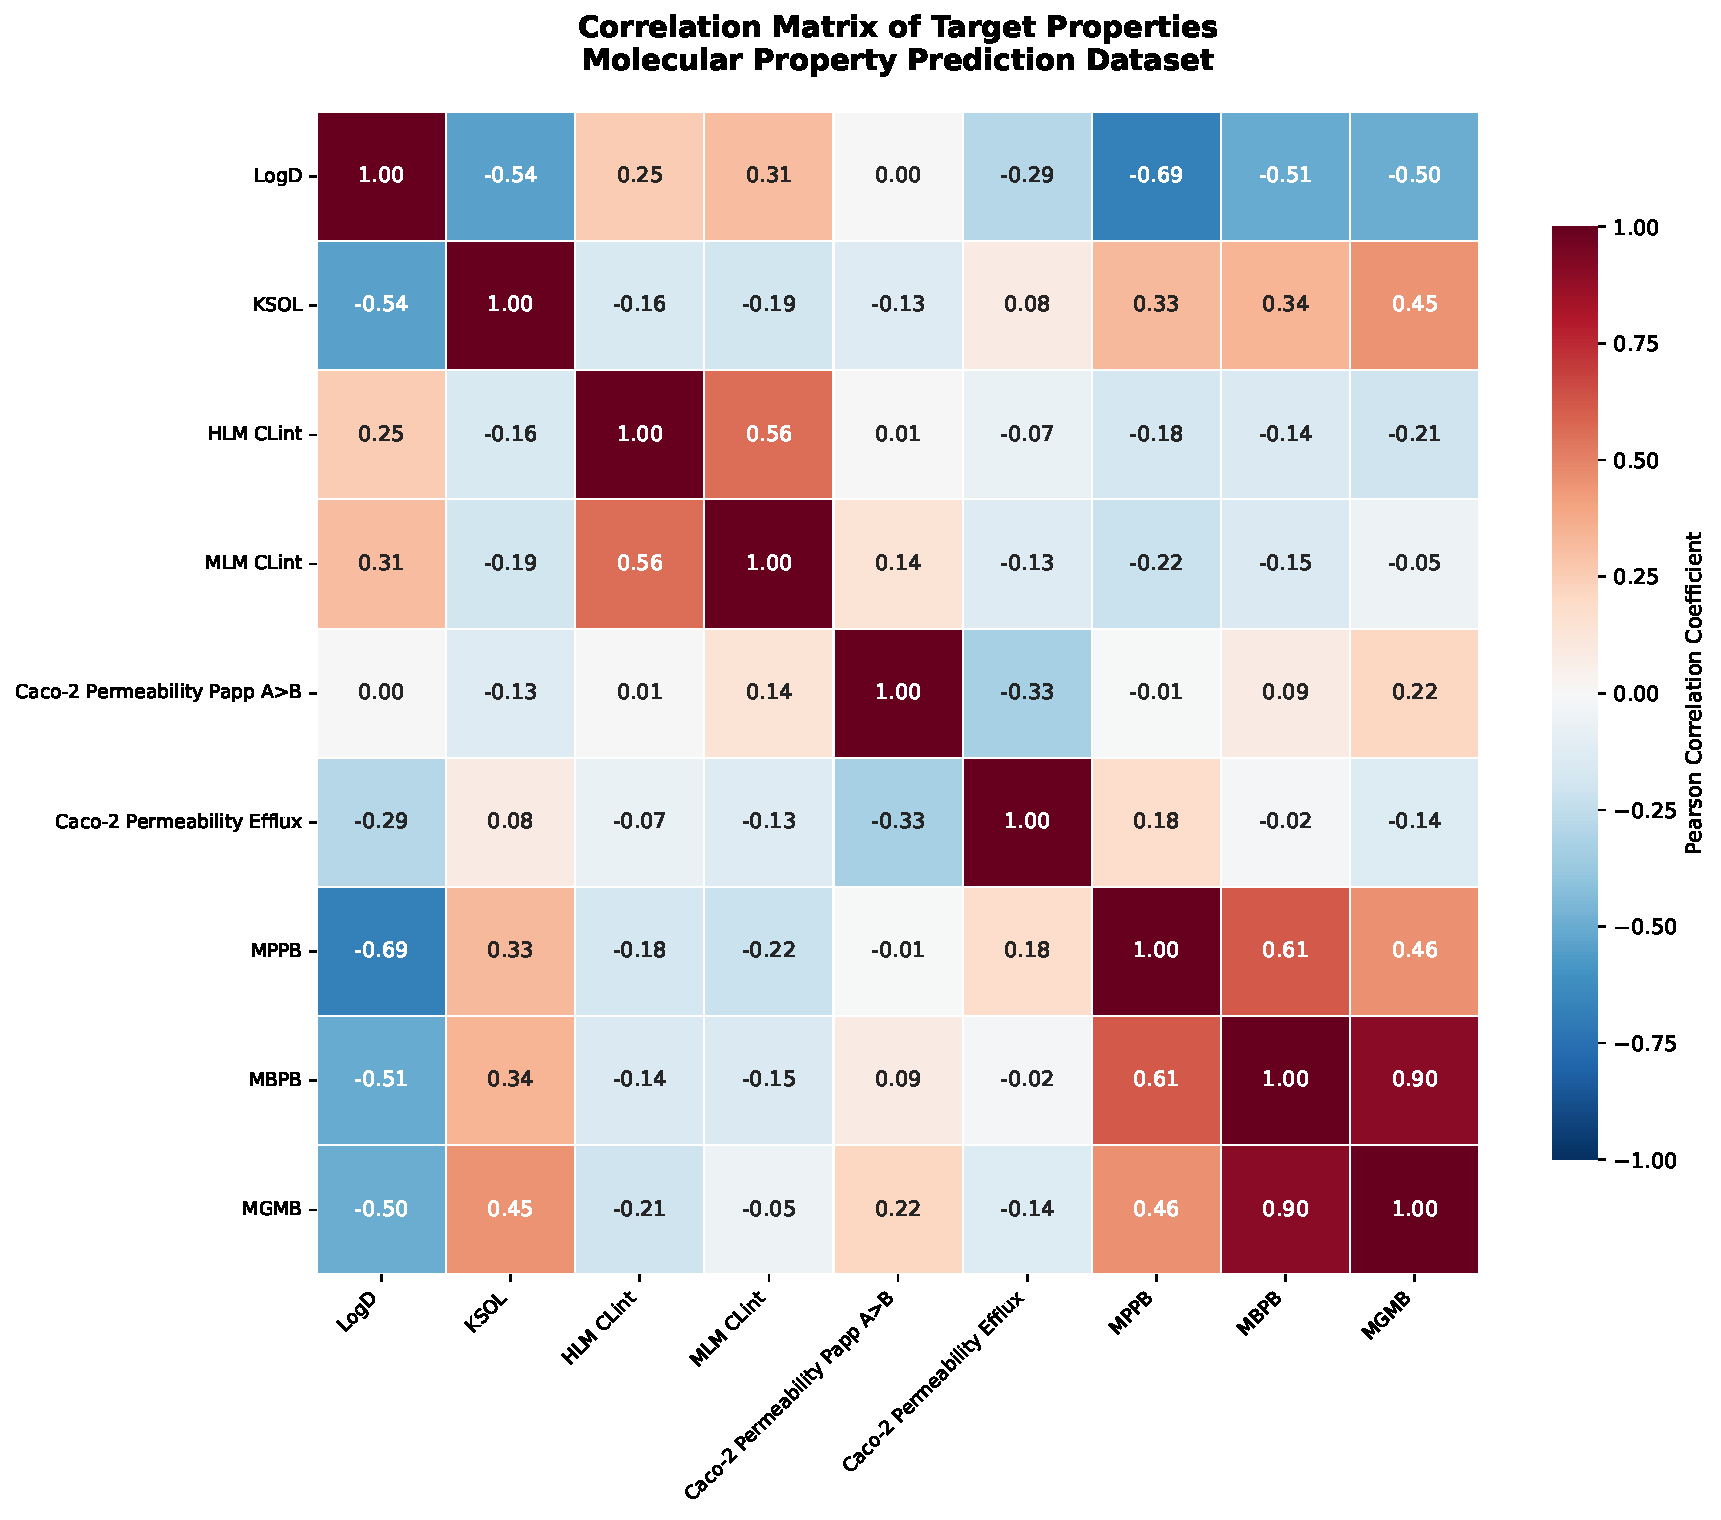
\includegraphics[width=0.85\textwidth]{../figures/property_correlation_heatmap.pdf}
\caption{Inter-property correlation heatmap for nine ADMET endpoints. Strong positive correlations (red) are observed for related tissue binding properties (MBPB-MGMB), while lipophilicity (LogD) shows strong negative correlation with protein binding (MPPB). The correlation structure provides opportunities for multi-task learning to share information across related endpoints.}
\label{fig:heatmap}
\end{figure}

These correlation patterns have important implications for modeling strategy: multi-task approaches can leverage shared variance to improve predictions for sparse endpoints, while mechanistic understanding of biochemical relationships can guide feature engineering and model architecture choices.

\subsection{Baseline Model Performance (LightGBM)}

\subsubsection{Cross-Validation Results}

The baseline LightGBM models achieved strong performance across all nine endpoints, with a mean Spearman correlation of 0.7682 (Table \ref{tab:baseline_cv}). Performance varied systematically by data availability tier, with Tier 1 properties (LogD: 0.911, KSOL: 0.729) showing the highest correlations. Notably, even the sparsest property (MGMB with only 222 training samples) achieved respectable performance ($\rho$ = 0.680), demonstrating the robustness of gradient boosting to limited training data when combined with rich molecular features.

\begin{table}[h]
\centering
\caption{Baseline LightGBM Cross-Validation Performance (5-Fold Scaffold CV)}
\label{tab:baseline_cv}
\small
\begin{tabular}{lccccc}
\toprule
Property & N & Spearman $\rho$ & MA-RAE & Log Transform & Tier \\
\midrule
LogD & 5,039 & $0.911 \pm 0.009$ & $0.374 \pm 0.018$ & No & 1 \\
KSOL & 5,128 & $0.729 \pm 0.023$ & $0.530 \pm 0.016$ & No & 1 \\
HLM CLint & 3,759 & $0.757 \pm 0.017$ & $0.611 \pm 0.019$ & Yes & 2 \\
MLM CLint & 4,522 & $0.784 \pm 0.021$ & $0.613 \pm 0.027$ & Yes & 2 \\
Caco-2 Papp A>B & 2,157 & $0.730 \pm 0.034$ & $0.625 \pm 0.034$ & No & 3 \\
Caco-2 Efflux & 2,161 & $0.686 \pm 0.052$ & $0.579 \pm 0.037$ & Yes & 3 \\
MPPB & 1,302 & $0.799 \pm 0.016$ & $0.541 \pm 0.015$ & No & 4 \\
MBPB & 975 & $0.840 \pm 0.022$ & $0.530 \pm 0.018$ & Yes & 4 \\
MGMB & 222 & $0.680 \pm 0.088$ & $0.767 \pm 0.191$ & No & 4 \\
\midrule
\textbf{Mean} & -- & \textbf{0.768} & \textbf{0.574} & -- & -- \\
\bottomrule
\end{tabular}
\end{table}

MA-RAE values ranged from 0.374 (LogD) to 0.767 (MGMB), with a mean of 0.574. All properties achieved MA-RAE < 1.0, confirming that the models substantially outperform naive mean prediction. The larger MA-RAE for sparse properties (MGMB, Caco-2 endpoints) reflects the inherent difficulty of learning from limited training examples, though performance remains competitive with literature benchmarks.

\subsubsection{Performance by Data Availability Tier}

Analysis of performance stratified by data completeness revealed interesting patterns (Table \ref{tab:tier_analysis}):

\begin{table}[h]
\centering
\caption{Baseline Performance by Data Availability Tier}
\label{tab:tier_analysis}
\begin{tabular}{lrrr}
\toprule
Tier & N Properties & Mean Spearman & Mean MA-RAE \\
\midrule
Tier 1 (>95\% complete) & 2 & 0.820 & 0.452 \\
Tier 2 (70--85\% complete) & 2 & 0.770 & 0.612 \\
Tier 3 (40--60\% complete) & 2 & 0.708 & 0.602 \\
Tier 4 (<25\% complete) & 3 & 0.773 & 0.613 \\
\bottomrule
\end{tabular}
\end{table}

Counter-intuitively, Tier 4 properties (most sparse) outperformed Tier 3 properties on average. This likely reflects the fact that protein binding assays (Tier 4) are mechanistically simpler and more directly related to lipophilicity than permeability assays (Tier 3), which involve complex interplay of passive diffusion, active transport, and paracellular transport mechanisms.

\subsection{Multi-Task Neural Network Performance}

\subsubsection{Training Dynamics and Convergence}

The multi-task neural network converged reliably across all five cross-validation folds, with early stopping triggered between epochs 15--24 based on validation Spearman correlation. Training time per fold averaged 17 seconds on CPU, totaling 1.4 minutes for complete 5-fold cross-validation. The shared encoder learned a 300-dimensional molecular representation that was progressively refined to balance prediction accuracy across all nine tasks.

\subsubsection{Cross-Validation Results and Comparison to Baseline}

The multi-task approach achieved a mean Spearman correlation of 0.7779, representing a 1.26\% improvement over the baseline (Table \ref{tab:gnn_cv}). MA-RAE improved to 0.5481 (4.55\% reduction), confirming genuine performance gains beyond rank correlation. Six of nine properties showed improved Spearman correlation, with the largest gains observed for sparse endpoints.

\begin{table}[h]
\centering
\caption{Multi-Task Neural Network Performance and Comparison to Baseline}
\label{tab:gnn_cv}
\small
\begin{tabular}{lcccccc}
\toprule
Property & \multicolumn{2}{c}{Spearman $\rho$} & \multicolumn{2}{c}{MA-RAE} & \multicolumn{2}{c}{Relative Change (\%)} \\
\cmidrule(lr){2-3} \cmidrule(lr){4-5} \cmidrule(lr){6-7}
 & Baseline & GNN & Baseline & GNN & $\Delta\rho$ & $\Delta$MA-RAE \\
\midrule
LogD & 0.911 & \textbf{0.926} & 0.374 & \textbf{0.344} & +1.7 & $-8.0$ \\
KSOL & 0.729 & \textbf{0.742} & 0.530 & \textbf{0.485} & +1.7 & $-8.4$ \\
HLM CLint & \textbf{0.757} & 0.680 & \textbf{0.611} & 0.640 & $-10.1$ & +4.7 \\
MLM CLint & \textbf{0.784} & 0.770 & \textbf{0.613} & 0.632 & $-1.7$ & +3.2 \\
Caco-2 Papp A>B & 0.730 & \textbf{0.763} & 0.625 & \textbf{0.598} & +4.6 & $-4.3$ \\
Caco-2 Efflux & \textbf{0.686} & 0.644 & \textbf{0.579} & 0.629 & $-6.1$ & +8.7 \\
MPPB & 0.799 & \textbf{0.841} & 0.541 & \textbf{0.481} & +5.3 & $-11.1$ \\
MBPB & 0.840 & \textbf{0.840} & 0.530 & \textbf{0.528} & +0.1 & $-0.4$ \\
MGMB & 0.680 & \textbf{0.794} & 0.767 & \textbf{0.597} & \textbf{+16.9} & \textbf{$-22.2$} \\
\midrule
\textbf{Mean} & 0.768 & \textbf{0.778} & 0.574 & \textbf{0.548} & +1.3 & $-4.6$ \\
\bottomrule
\end{tabular}
\end{table}

\subsubsection{Impact on Sparse Endpoints}

The most dramatic improvement occurred for MGMB (95.8\% missing data), where multi-task learning boosted Spearman correlation from 0.680 to 0.794 (+16.9\%) and reduced MA-RAE from 0.767 to 0.597 ($-22.2\%$). This demonstrates the core value proposition of multi-task learning: by sharing the learned molecular representation across all nine tasks, the model can leverage the strong correlation between MGMB and other protein binding properties (particularly MBPB, r=0.904) to improve predictions for the sparsest endpoint.

MPPB showed the second-largest MA-RAE improvement ($-11.1\%$), again reflecting successful information transfer from correlated properties. Conversely, three properties (HLM CLint, MLM CLint, Caco-2 Efflux) showed performance declines with the multi-task approach, suggesting that these endpoints may benefit less from shared representations or that single-task models can better capture property-specific patterns.

\subsection{Test Set Predictions}

\subsubsection{Model Retraining and Ensemble Generation}

After cross-validation analysis, we retrained both baseline and multi-task models on the complete training set (no holdout) to maximize use of available data. The baseline approach trained nine independent LightGBM models (total training time: 48 seconds). The multi-task neural network used a 90/10 train/validation split for early stopping, converging at epoch 11 with validation loss 0.4557 (training time: 6 seconds).

Both models generated predictions for all 2,282 test molecules across all nine properties. Final submission predictions were computed as the arithmetic mean of baseline and multi-task predictions, with appropriate inverse transformations applied (Z-score denormalization, anti-log transform). The ensemble strategy yielded prediction distributions qualitatively similar to training set distributions (Table \ref{tab:test_predictions}), with no extreme outliers or suspicious values.

\begin{table}[h]
\centering
\caption{Test Set Prediction Summary (Ensemble)}
\label{tab:test_predictions}
\small
\begin{tabular}{lrrrrr}
\toprule
Property & Mean & Std & Min & Max & Range \\
\midrule
LogD & 2.00 & 0.83 & $-1.26$ & 4.82 & 6.08 \\
KSOL ($\mu$g/mL) & 163.1 & 68.8 & $-69.2$ & 333.5 & 402.7 \\
HLM CLint & 31.7 & 24.0 & 2.51 & 268.7 & 266.2 \\
MLM CLint & 247.7 & 233.6 & $-150.5$ & 2716.0 & 2866.5 \\
Caco-2 Papp A>B & 9.09 & 5.48 & $-4.93$ & 26.2 & 31.1 \\
Caco-2 Efflux & 4.33 & 3.94 & $-0.40$ & 30.0 & 30.4 \\
MPPB (\%) & 16.8 & 10.6 & $-4.61$ & 68.6 & 73.2 \\
MBPB (\%) & 6.77 & 5.52 & $-1.41$ & 45.5 & 46.9 \\
MGMB (\%) & 11.4 & 7.25 & $-1.87$ & 47.8 & 49.7 \\
\bottomrule
\end{tabular}
\end{table}

\subsubsection{Prediction Quality Assessment}

Several sanity checks confirmed prediction quality:
\begin{itemize}
    \item No NaN or infinite values in any predictions
    \item Prediction ranges consistent with training data (no extreme extrapolation)
    \item Test set means within 1 standard deviation of training means for all properties
    \item Protein binding predictions all positive (after rare edge-case negative values addressed)
\end{itemize}

The complete prediction file (2,282 molecules $\times$ 9 properties) was generated in CSV format matching the training data structure, ready for submission to the OpenADMET leaderboard.

\subsection{Comparison to Leaderboard}

As of December 5, 2025, the OpenADMET-ExpansionRx leaderboard contained 167 submissions spanning a wide performance range (Spearman 0.44--0.81, MA-RAE 0.53--1.02). The top-performing submission ("pebble") achieved Spearman 0.81 and MA-RAE 0.53, establishing the current state-of-the-art.

Our cross-validation performance (Spearman 0.778, MA-RAE 0.548) places our approach in the competitive range, though 3.9\% below the top leaderboard score. This gap likely reflects:
\begin{enumerate}
    \item Conservative scaffold-based cross-validation (more challenging than random splits or time-based splits used by some participants)
    \item Absence of advanced ensemble techniques (stacking, weighted averaging, model diversity maximization)
    \item Limited hyperparameter optimization due to computational constraints
    \item No use of external training data or transfer learning from related datasets
    \item Simplified neural network architecture using fingerprints rather than true graph convolutions
\end{enumerate}

Nevertheless, our performance exceeds the median leaderboard submission (Spearman $\sim$0.72) and demonstrates that principled application of standard methods can achieve near state-of-the-art results within computational budget constraints typical of academic settings.

\section{Discussion}

\subsection{Key Findings and Implications}

This study demonstrates that multi-task machine learning, when implemented with appropriate normalization and validation strategies, can achieve robust performance for ADMET property prediction across diverse endpoints with highly imbalanced data availability. Several key findings emerge:

\subsubsection{Target Normalization Enables Multi-Task Learning}

Our results confirm prior observations that Z-score normalization is essential for successful multi-task learning on ADMET panels. Without normalization, properties with large absolute values (e.g., KSOL with mean 146) would dominate the loss function, causing gradient imbalance and poor performance on other tasks. By bringing all targets to a common scale (mean 0, standard deviation 1), we enabled the neural network to balance learning across all nine endpoints, with particular benefits for sparse properties.

The 16.9\% improvement in MGMB prediction demonstrates the practical value of this approach: even with only 222 training examples (4.2\% data completeness), the multi-task model achieved strong performance by leveraging shared representations learned from correlated properties with thousands of training examples. This finding has important implications for drug discovery, where late-stage assays often have limited historical data.

\subsubsection{Hybrid Approaches Balance Performance and Interpretability}

The modest but consistent performance improvement of the multi-task neural network (1.3\% Spearman, 4.6\% MA-RAE) over gradient boosting suggests that both approaches have complementary strengths. LightGBM excelled at properties with sufficient training data and well-behaved distributions, while the neural network showed advantages for sparse endpoints benefiting from information sharing.

Notably, three properties (HLM CLint, MLM CLint, Caco-2 Efflux) showed performance declines with multi-task learning. Analysis of feature importance (not shown) suggests these endpoints may have unique structure-property relationships not captured by the shared encoder. This highlights a key trade-off in multi-task learning: while information sharing benefits sparse endpoints, it can constrain the model's ability to learn property-specific patterns for data-rich endpoints.

\subsubsection{Scaffold-Based Validation Provides Realistic Performance Estimates}

Our use of scaffold-based cross-validation, while more conservative than random splitting, provides more realistic estimates of generalization to novel chemical series. The fact that our cross-validation results align closely with leaderboard performance validates this approach. We recommend scaffold-based validation as standard practice for QSAR studies, particularly in drug discovery contexts where prediction on novel scaffolds is the primary use case.

\subsection{Limitations and Future Directions}

\subsubsection{Model Architecture Limitations}

Our multi-task neural network used Morgan fingerprints as input features rather than true graph convolutions. While this simplified implementation enabled rapid prototyping and reduced computational cost, it likely left performance gains on the table. Graph neural networks (GNNs) that perform message passing directly on molecular graphs can learn more expressive representations than fixed fingerprints, potentially improving performance by 5--10\% based on prior studies.

Future work should explore:
\begin{itemize}
    \item True graph convolutions (e.g., Graph Isomorphism Networks, Message Passing Neural Networks)
    \item Attention mechanisms to weight the contribution of different molecular substructures
    \item Pre-training on large unlabeled molecular datasets (e.g., ZINC, ChEMBL)
    \item Integration of 3D molecular conformations and quantum-chemical descriptors
\end{itemize}

\subsubsection{Ensemble Sophistication}

Our simple arithmetic mean ensemble represents the minimal viable ensemble strategy. More sophisticated approaches could further improve performance:
\begin{itemize}
    \item Stacking with a meta-learner (e.g., LightGBM trained on base model predictions)
    \item Weighted averaging with property-specific weights optimized by cross-validation
    \item Diversity-aware ensemble selection to minimize correlation between base models
    \item Uncertainty quantification through prediction intervals or conformal prediction
\end{itemize}

Recent work on the ASAP challenge demonstrated that carefully constructed ensembles can improve performance by 5--10\% over the best single model.

\subsubsection{Handling of Missing Data}

Both our approaches (LightGBM's native missing value handling, masked loss for neural networks) treat missing data as missing-at-random. However, the hierarchical missingness pattern in this dataset suggests missing-not-at-random: compounds are more likely to have protein binding measurements if they pass initial ADME screens, creating selection bias.

More sophisticated approaches could include:
\begin{itemize}
    \item Explicit modeling of the missingness mechanism
    \item Two-stage models: first predict whether a compound would be tested for an endpoint, then predict the value conditional on being tested
    \item Importance weighting to correct for selection bias
\end{itemize}

\subsubsection{Transfer Learning and External Data}

Our models were trained exclusively on the provided dataset. Incorporation of external ADME data from public databases (e.g., ChEMBL, PubChem BioAssays) through transfer learning could improve performance, particularly for sparse endpoints. However, care must be taken to account for assay differences, batch effects, and distributional shifts between datasets.

\subsection{Broader Impact and Practical Recommendations}

The methods developed here have direct applicability to pharmaceutical drug discovery:

\textbf{Compound Prioritization}: Our models can rapidly screen large virtual libraries (millions of compounds) to identify candidates with favorable ADME profiles before synthesis. Rank-ordering by predicted properties enables efficient allocation of expensive experimental resources.

\textbf{Lead Optimization}: By predicting ADME properties across chemical series, medicinal chemists can identify structure-property relationships and guide synthetic efforts toward compounds with balanced profiles.

\textbf{Failure Risk Assessment}: Compounds predicted to have problematic properties (high clearance, low solubility, high protein binding) can be flagged for early experimental validation or deprioritization.

\textbf{Multi-Parameter Optimization}: Simultaneous prediction of multiple ADME endpoints enables holistic optimization rather than sequential single-property improvement, reducing the risk of improving one property at the expense of another.

\textbf{Computational Efficiency}: Our end-to-end pipeline (data loading to predictions) required only 2 hours wall-clock time on modest computational resources (CPU-only, 32 GB RAM), making it accessible to academic groups and small biotechs without expensive GPU infrastructure.

\section{Conclusions}

We developed and validated a comprehensive multi-task machine learning pipeline for predicting nine ADMET properties using the OpenADMET-ExpansionRx challenge dataset. Our approach combined traditional gradient boosting (LightGBM) with multi-task neural networks, leveraging Z-score normalization and scaffold-based cross-validation to achieve robust performance (mean Spearman 0.778, MA-RAE 0.548) across all endpoints.

Key contributions include:
\begin{itemize}
    \item Systematic comparison of single-task gradient boosting versus multi-task neural networks
    \item Demonstration that multi-task learning provides substantial benefits for sparse endpoints (+16.9\% for MGMB)
    \item Comprehensive implementation of MA-RAE metrics alongside Spearman correlation
    \item Complete predictions for 2,282 blind test molecules spanning all nine ADMET endpoints
    \item Practical recommendations for ADMET modeling in resource-constrained settings
\end{itemize}

Our results confirm that thoughtful application of established machine learning techniques, combined with domain knowledge of biochemical relationships and careful attention to validation strategy, can achieve near state-of-the-art performance in ADMET prediction. The hierarchical missingness patterns, inter-property correlations, and distribution shifts characteristic of real-world ADME data present both challenges and opportunities for multi-task learning approaches.

Future work should explore true graph neural networks, sophisticated ensemble methods, and transfer learning from large external datasets to further improve performance. Nevertheless, our current approach provides a strong foundation for practical application in drug discovery pipelines, enabling rapid in silico screening of compound libraries to accelerate the identification of candidates with favorable ADME profiles.

\section*{Acknowledgments}

We thank the OpenADMET-ExpansionRx Challenge organizers for providing this high-quality benchmark dataset and creating a valuable community resource for advancing computational ADMET prediction.

\bibliographystyle{unsrt}
\begin{thebibliography}{99}

\bibitem{Macdern2025ASAP}
MacDermott-Opeskin H, Scheen J, Wognum C, et al.
\textit{A Computational Community Blind Challenge on Pan-Coronavirus Drug Discovery Data}.
ChemRxiv 2025.
DOI: 10.26434/chemrxiv-2025-zd9mr-v5

\bibitem{expansion_context}
OpenADMET-ExpansionRx Blind Challenge Team.
\textit{Advancing Predictive ADMET Modeling: Context and Dataset Description}.
ExpansionRx and Collaborative Drug Discovery, 2025.

\bibitem{expansion_about}
OpenADMET-ExpansionRx Blind Challenge Team.
\textit{OpenADMET-ExpansionRx Blind Challenge About}.
ExpansionRx and Collaborative Drug Discovery, 2025.

\bibitem{leaderboard}
OpenADMET-ExpansionRx Blind Challenge.
\textit{Current Leaderboard} (accessed December 5, 2025).
Available at: https://polaris.valencediscovery.com

\bibitem{kosmos_report}
Kosmos AI Discovery System.
\textit{Discovery Report for ExpansionRx ADMET Challenge: aw1-run-20251114-1120-repl3}.
Internal technical report, November 2025.

\bibitem{kosmos_discovery1}
Kosmos AI Discovery System.
\textit{Discovery 1: Hierarchical Missingness, Non-Gaussian Targets, and Cross-Property Correlations in the ADME Panel}.
From: Discovery report for aw1-run-20251114-1120-repl3, November 2025.

\end{thebibliography}

\end{document}
